\documentclass[11pt]{llncs}
\usepackage{preamble}

\begin{document}
\import{./}{title.tex}
\thispagestyle{plain}
\import{./}{abstract.tex}
\import{./}{introduction.tex}
\import{./}{oracle.tex}

\section{Constructing non-interactive proofs}

A non-interactive proof-of-proof of work is a game between a Prover and a
Verifier parameterized by predicate $q$ which the prover tries to convience the
verifier for. The predicate $q$ is a function of a chain $\chain$, which the
prover claims to be the longest chain.

\import{./}{algorithms/alg.backbone.tex}
\import{./}{algorithms/alg.verifier-framework.tex}
\import{./}{algorithms/alg.verifier-full.tex}
\import{./}{algorithms/alg.verifier-lite.tex}

At the beginning of the game, two Provers generate proofs $\pi_A$, $\pi_B$
claiming potentially different truth values for the predicate $q$ based on
their claimed local longest chains. The Verifier receives these proofs and
accepts one of the two proofs, determining the truth value of the predicate.

\section{Provable chain predicates}

We now describe the desirable property of predicates, \textit{monotonicity},
which is an adequate condition to show that the predicats are provable. Based
on predicate monotonicity, we show that a predicate has \textit{liveness} and
\textit{persistence} and define chain predicate security appropriately.

We allow our predicates to have an undefined value $\bot$ before they take
on a truth value of $0$ or $1$.

\begin{definition}{(Predicate monotonicity)}
    A chain predicate $Q(\chain)$ is $\textit{monotonous}$ if for all chains
    $\chain$ and for all blocks $B$ we have that:

    \begin{equation*}
        Q(\chain) \neq \bot \Rightarrow Q(\chain) = Q(\chain B)
    \end{equation*}
\end{definition}

\begin{definition}{(Predicate switching position)}
    A chain predicate $Q(\chain) \neq \bot$ has a switching position $i \in
    \mathbb{N}$ in the chain $\chain$ defined as the minimum $i$ such that:

    \begin{equation*}
        Q(\chain^{\rest |\chain| - i}) \neq \bot
    \end{equation*}
\end{definition}

\begin{definition}{(Predicate stability)}
    Parameterized by $k \in \mathbb{N}$, a chain predicate $Q(\chain)$ has
    $\textit{stability}$ if its switching position $i$ satisfies $i < |\chain|
    - k$.
\end{definition}

\begin{definition}{(Predicate persistence)}
    Parameterized by $k \in \mathbb{N}$, a chain predicate $Q(\chain)$ has
    $\textit{persistence}$ if the following is true: When in a certain round
    the predicate is $k$-stable in some honest party's chain, then whenever it is
    $k$-stable in any honest party's chain, the truth value of the predicate is
    the same. Furthermore, the change of truth value from $\bot$ to its final
    truth value happened at the same blockchain depth.
\end{definition}

\begin{definition}{(Predicate liveness)}
    Parameterized by $u, k \in \mathbb{N}$ (the ``wait time'' and ``depth''
    parameters respectively), a chain predicate $Q(\chain)$ has
    $\textit{liveness}$ if it is $k$-stable for one honest part in a certain
    round, then it will also be $k$-stable for all honest parties after $u$ rounds.
\end{definition}

\begin{theorem}
    If a chain predicate is monotonous, then it satisfies persistence with
    parameter $k = 2\eta \kappa f$ with probability at least $1 -
    e^{-\Omega(\kappa)}$.
\end{theorem}

\begin{proof}
    Assume a typical execution and let $\chain_1$ be the chain of some honest
    player $P_1$ at round $r_1$. Assume that the chain predicate $Q(\chain)$ is
    $k$-stable for $P_1$ at round $r_1$, i.e.  $Q(\chain^{\rest k}) \neq \bot$.
    The chain of any honest player $P_2$ will be at least as long from the next
    round on and from common prefix we have that $\chain_1^{\rest k}
    \preccurlyeq \chain_2$. Therefore the predicate will be $k$-stable, have
    the same truth value, and have the same switching position for all honest
    parties.
\end{proof}

\begin{theorem}
    If a chain predicate is monotonous, then it satisfies liveness with
    parameters $u = 4\eta(1 - \epsilon)^{-1}\kappa$ rounds and $k = 2\eta
    \kappa f$ with probability at least $1 - e^{-\Omega(\kappa)}$.
\end{theorem}

\begin{proof}
    ?
\end{proof}

\import{./}{algorithms/alg.nipopow-innerchain.tex}

We introduce a helper algorithm, ConstructInnerChain, shown in
Algorithm~\ref{alg.nipopow_construct_innerchain}. This algorithm returns the innerchain
of level $i$ extracted from the blockchain $\chain$. If boundary is provided,
it only returns the blocks more recent than the boundary block supplied.

\import{./}{algorithms/alg.nipopow-prover.tex}

The NiPoPoW proof construction is shown in Algorithm~\ref{alg.nipopow_construct_proof}.
This produces a non-interactive PoPoW in parameter $m$ which consists of a
number of blocks for every level $i$. The number of blocks per level is
approximately $2m$.

\begin{figure}[h]
    \caption{The hierarchical blockchain. Existing blocks are shown in level 1.
    Higher levels have achieved a lower target (higher difficulty) during mining.}
    \centering
    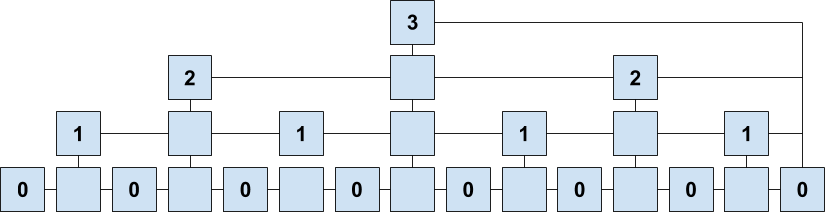
\includegraphics[width=\textwidth,keepaspectratio]{figures/hierarchical-ledger.png}
    \label{fig:hierarchy}
\end{figure}

\begin{figure}[h]
    \caption{The first of a series of interactive proofs-of-proofs-of-work for
    $m = k = 3$. This proof is the only one that needs to be sent in case it
    goes unchallenged.}
    \centering
    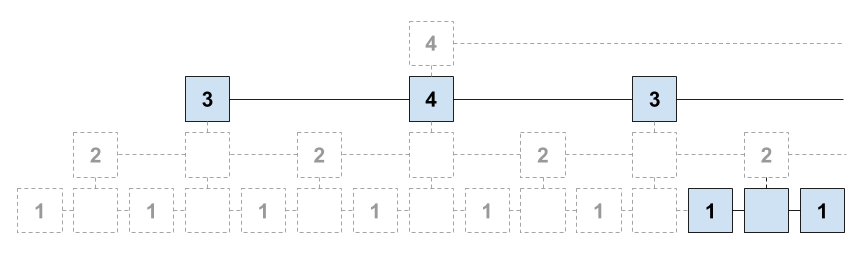
\includegraphics[width=\textwidth,keepaspectratio]{figures/interactive-popow.png}
\end{figure}

\begin{figure}[h]
    \caption{A non-interactive proof-of-work for $m = k = 3$. Any challenges
    can be answered by the verifier directly by constructing a proof from the
    data in this proof, without interaction with the prover.}
    \centering
    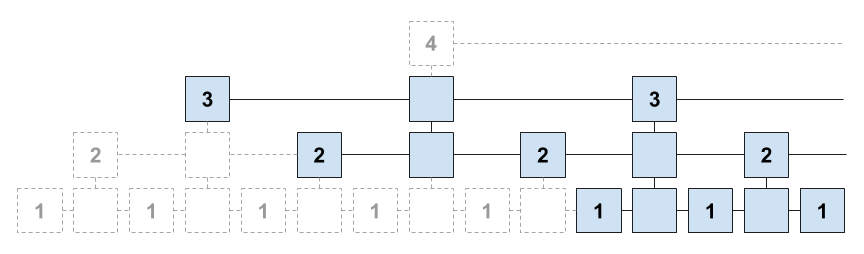
\includegraphics[width=\textwidth,keepaspectratio]{figures/non-interactive-popow.png}
\end{figure}

\import{./}{references.tex}
\end{document}
